\lstinputlisting[language=bash,basicstyle=\small]{python_codes/fieldstone_70/keywords}

\begin{center}
Code at \url{https://github.com/cedrict/fieldstone/tree/master/python_codes/fieldstone_70}
\end{center}

\par\noindent\rule{\textwidth}{0.4pt}

%%%%%%%%%%%%%%%%%%%%%%%%%%%%%%%%%%%%%%%%%%%%%%%%%%%%%%%%%%%%%%%%%%%%%%%%%%%%%%%%%%%%%%%%%%%%%%%%%%%%

The setup is borrowed from Duretz et al (2020) \cite{dudy20}. 
Two major differences with the paper: 1) no elasticity and 2) no Newton solver.

The model consists of a $100\times 30\si{km}$ slice of Westerly Granite (Hansen \& Carter, 1983), 
which comprises an imperfection at the center of the domain.
This weak inclusion with a $2\si{km}$ radius serves to initiate
localized deformations. The model configuration is thus perfectly symmetric. 
The model includes a vertical temperature gradient ($-15\si{\celsius\per\km}$) (starting 
at $20\si{\celsius}$ at the surface), 
a constant density ($2700\si{\kg\per\cubic\metre}$), and the acceleration of gravity ($g_y=-10\si{\metre\per\second\squared}$).
The inclusion is characterised by $\eta=10^{20}\si{\pascal\second}$.
The domain is subjected to kinematic boundary conditions, which cause a pure shear stress state:

\begin{center}
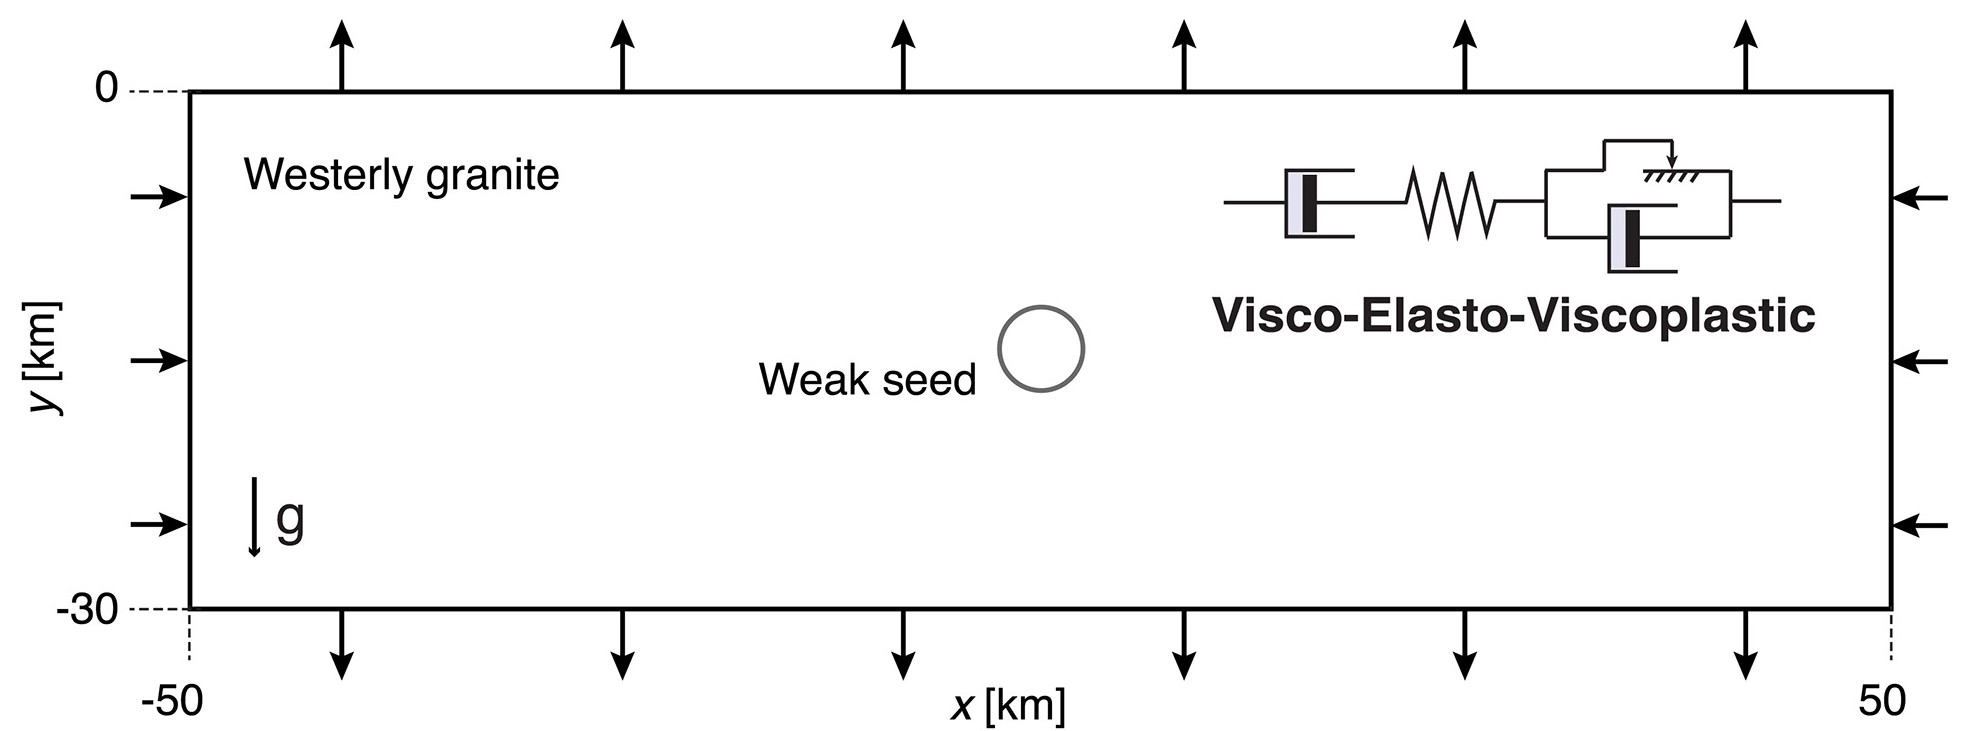
\includegraphics[width=12cm]{python_codes/fieldstone_70/images/fig1}\\
{\captionfont Figure taken from \cite{dudy20}}
\end{center}

All boundaries are free slip. The material can behave in a ductile manner in the lower, hot
part of the domain (displaying temperature-dependent power law creep), and in a viscoplastic 
manner in the upper, cold part of the domain. The parameters are 
$A=3.1623\cdot 10^{-26}\si{\pascal^{-n}\per\second}$, 
$Q=186.5\cdot 10^3 \si{\joule\per\mole}$, 
$n=3.3$, $c=50\si{\mega\pascal}$, $\phi=\arctan(0.6)\simeq 31\degree$ and $\eta^{vp}=10^{21}\si{\pascal\second}$

The background strainrate is set such that $\dot{\varepsilon}_{bc}=10^{-15}\si{\per\second}$, i.e. 
$v_{bc}=\pm \dot{\varepsilon}_{bc} L_x/2 $ on the sides and $v=\pm \dot{\varepsilon}_{bc} L_y/2 $
on the top and bottom boundaries. Pressure is normalised such that it is on average zero on the top boundary. 
Picard iterations are used. The 2-norm of the non-linear residual 
is monitored, as well as the following quantities ($i$ and $i-1$ are two consecutive nonlinear iterations):
\[
\xi_u = \frac{\|u^i-u^{i-1}\|_2}{ \|u^i+u^{i-1}\|_2}
\qquad
\qquad
\xi_v = \frac{\|v^i-v^{i-1}\|_2}{ \|v^i+v^{i-1}\|_2}
\qquad
\qquad
\xi_p = \frac{\|p^i-p^{i-1}\|_2}{ \|p^i+p^{i-1}\|_2}
\] 

As shown on the (modified) figure above, the rheological assemblage is as follows:
\begin{center}
\begin{flushright} {\tiny {\color{gray} (tikz\_vvp.tex)}} \end{flushright}
%~~~~~~~~~~~~~~~~~~~~~~~~~~~~~~~~~~~~~~~~~~~~~~~~~~~~~~~~~~~~~~~~~~~~~~~~~~~~~~~~~~~~~~~~~~~~~~~~~~

\begin{center}
\begin{tikzpicture}
%\draw[fill=gray!23,gray!23](0,0) rectangle (7,5);
%\draw[step=0.5cm,gray,very thin] (0,0) grid (7,5); %background grid

\node[] at (0.1,2.7) {$\tau$};
\draw[line width=1mm] (0.5,1.5) -- (0.5,3.5) ;  
\draw [->] (0,2.5) -- (0.45,2.5);
\draw [->] (0,2) -- (0.45,2);
\draw [->] (0,3) -- (0.45,3);

\draw[thick] (0.5,2.5) -- (2,2.5) ;  
\draw[thick] (2.5,2.5) -- (4.5,2.5) ;  
\draw[thick] (7.5,2.5) -- (9,2.5) ;  

\draw[thick] (1.5,3) -- (2.5,3) -- (2.5,2) -- (1.5,2);  
\draw[thick] (5.5,4) -- (6.5,4) -- (6.5,3) -- (5.5,3);  

\node[] at (2,1.6) {$\eta_v$};
\node[] at (6,4.4) {$\eta_m$};

\draw[thick] (6,3.5) -- (4.5,3.5) -- (4.5,1.5) -- (5,1.5);  
\draw[thick] (6.5,3.5) -- (7.5,3.5) -- (7.5,1.5) -- (7,1.5);  

\draw[thick] (5,1.5) -- (5.5,1.4) -- (6.5,1.4) ;  
\draw[thick] (5.5,1.6) -- (6.5,1.6) -- (7,1.5) ;  

\node[] at (6,1.92) {$Y$};

%wall
\draw[line width=2mm] (9,1.5) -- (9,3.5) ;  
\draw[thick] (9,1.5) -- (9.25,1.75) ;  
\draw[thick] (9,1.75) -- (9.25,2) ;  
\draw[thick] (9,2) -- (9.25,2.25) ;  
\draw[thick] (9,2.25) -- (9.25,2.5) ;  
\draw[thick] (9,2.5) -- (9.25,2.75) ;  
\draw[thick] (9,2.75) -- (9.25,3) ;  
\draw[thick] (9,3) -- (9.25,3.25) ;  
\draw[thick] (9,3.25) -- (9.25,3.5) ;  

\draw[>=triangle 45, <->] (0.5,0.95) -- (3.5,0.95);
\draw[>=triangle 45, <->] (3.5,0.95) -- (9,0.95);
\node[] at (2,0.75)   {$\dot\varepsilon_{v}$};
\node[] at (6.5,0.75)   {$\dot\varepsilon_{vp}$};

\end{tikzpicture}
\end{center}

\end{center}

The dislocation creep viscosity $\eta_{\color{green}ds}$ and effective viscoplastic viscosity $\eta_{vp}$ are given by 
\[
\eta_{\color{green}ds}(\dot\varepsilon) = \frac{1}{2} A^{-1/n} \dot{\varepsilon}^{-1+1/n} \exp \frac{Q}{nRT}
\qquad
\text{and}
\qquad
\eta_{vp}(\dot\varepsilon) = \frac{p \sin \phi + c \cos \phi}{2 \dot{\varepsilon}}  + \eta_{vp}
\]
Note that these expressions are functions of $\dot\varepsilon$, the nature of which will be specified later. 
As documented in Section~\ref{ss:srpart}, 
the partitioning of the total strain rate into a viscous creep component and a viscoplastic component 
is not trivial.  
The algorithm goes then as follows:
\begin{enumerate}
\item Assume we know $\dot\varepsilon_T$ (from previous iteration), 
as well as the yield value  $Y = p\; \sin\phi + c \; \cos \phi$ and $\eta_m$.
\item We start by assuming that the plasticity 'block' is not active 
($\dot{\varepsilon}_{\color{blue}vp}=0$, $\dot{\varepsilon}_{\color{green}ds}=\dot{\varepsilon}_T$): 
We are left with only one damper and compute its effective viscosity
\[
\eta_{\color{green}ds} = \frac{1}{2} A^{-1/n} \dot{\varepsilon}_T^{-1+1/n} \exp \left( \frac{Q}{nRT} \right)
\] 

\item if $\tau =2 {\eta}_{\color{green}ds} \dot\varepsilon_T < Y$ the stress is below the yield stress value 
and the plasticity element is indeed not active. Simply return ${\eta}_{\color{green}ds}$ in the material model.

\item if $\tau=2 \eta_{\color{green}ds} \dot\varepsilon_T > Y$ the stress is above the 
yield value, which is not allowed. In this case the plastic element must be present 
and active and the dislocation creep viscous damper is then 
in series with the viscoplastic element. The former deforms 
with a strain rate $\dot{\varepsilon}_{\color{green}ds}$ while the latter 
with $\dot\varepsilon_{\color{blue}vp}$ (all under the same tress $\tau$) 
and we have  $\dot\varepsilon_T = \dot{\varepsilon}_{\color{green}ds} + \dot\varepsilon_{\color{blue}vp}$ so:

\begin{eqnarray}
\dot\varepsilon_T - \dot{\varepsilon}_{\color{green}ds}(\tau) 
&=& \dot\varepsilon_{\color{blue}vp}(\tau)  \nonumber\\
&=& \frac{\tau}{2 \eta_{\color{blue}vp}}  \nn\\
&=& \frac{\tau}{2 \left( \frac{Y}{2\dot\varepsilon_{\color{blue}vp}(\tau)} + \eta_m  \right)} 
\nonumber\\
%&=&  \frac{\tau}{2 \left( \frac{Y}{2 (\dot\varepsilon_T -\dot{\varepsilon}_v(\tau) -\dot\varepsilon_{ds}(\tau) 
%+ \dot\varepsilon_{df}(\tau)   )} + \eta_m  \right)} 
%\nonumber\\
\dot\varepsilon_T -  \dot{\varepsilon}_{\color{green}ds}(\tau) 
&=&
\frac{\tau}{2 \left( \frac{Y}{2 (\dot\varepsilon_T -\dot{\varepsilon}_v(\tau)  )} + \eta_m  \right)} \nonumber 
\\
2 [\dot\varepsilon_T -\dot{\varepsilon}_v(\tau)  ]
 \left( \frac{Y}{2 (\dot\varepsilon_T -\dot{\varepsilon}_{\color{green}ds}(\tau) )} + \eta_m  \right) &=& \tau 
\nonumber\\
Y + 2 (\dot\varepsilon_T - \dot{\varepsilon}_v(\tau)  -\dot{\varepsilon}_{\color{green}ds}(\tau) ) \eta_m  &=& \tau \nonumber 
\end{eqnarray}
As before, we must find the zero of the function ${\cal F}(\tau)$: 
\begin{eqnarray}
{\cal F}(\tau) 
&=& Y + 2 [\dot\varepsilon_T -\dot{\varepsilon}_v(\tau)   -\dot{\varepsilon}_{\color{green}ds}(\tau) ]\eta_m -\tau \nonumber\\
&=& Y + 2 \left[ 
\dot\varepsilon_T -\frac{\tau}{2\eta_v} -A \tau^n \exp \left(-\frac{Q}{RT}\right) 
\right]\eta_m -\tau \nn
\end{eqnarray}
Because dislocation creep involves the $n$-th power of the stress (and $n$ need not be an integer!) 
finding the value of the stress for which ${\cal F}=0$ is not straightforward.
This equation can be solved with a Newton-Raphson algorithm
and the iterations will be of the form:
\[
\tau_{n+1} = \tau_n - \frac{{\cal F}(\tau_n)}{{\cal F}'(\tau_n)}
\]
where the derivative of the function ${\cal F}$ with respect to $\tau$ reads:
\begin{eqnarray}
\frac{\partial {\cal F}}{\partial \tau} 
&=& -\frac{\eta_m}{\eta_v} -2 \eta_m \frac{\partial  \dot\varepsilon_{v}(\tau) }{\partial \tau}    - 1 
= -\frac{\eta_m}{\eta_v}-2 \eta_m n A \tau^{n-1} \exp \left(-\frac{Q}{RT}\right) -1 
\end{eqnarray}
{\it Say something about where we start from, multiplicity of roots}

{\it Say something about when we stop iterating}

\item Once $\tau$ has been found, one can compute 
\begin{eqnarray}
\dot{\varepsilon}_{ds}(\tau)&=&A \tau^n \exp \left(-\frac{Q}{RT}\right)
\qquad \Rightarrow \qquad 
\eta_{ds}(\dot\varepsilon_{ds}) = \frac{1}{2} A^{-1/n} \dot{\varepsilon}_{ds}^{-1+1/n} \exp \frac{Q}{nRT} \nn\\
\dot{\varepsilon}_{v}(\tau)=\frac{\tau}{2\eta_v}  \nn
\end{eqnarray}
then $\dot{\varepsilon}_{\color{blue}vp}=\dot{\varepsilon}_T -\dot{\varepsilon}_v(\tau) -\dot{\varepsilon}_{ds}(\tau)$,
and then 
\[
\eta_{\color{blue} vp}(\dot\varepsilon_{\color{blue} vp}) = \frac{p \sin \phi + c \cos \phi}{2 \dot{\varepsilon}_{\color{blue}vp}}  + \eta_{\color{blue} vp}
\]
\item 
Ultimately the effective viscosity at every quadrature point is computed as follows:
\[
\eta_{eff} = \left(\frac{1}{\eta_v} + \frac{1}{\eta_{ds}}  + \frac{1}{\eta_{vp}}  \right)^{-1}
\]
For the first nonlinear iteration there is no pre-existing velocity or pressure field so EXPLAIN 


\end{enumerate}



%I set $\dot{\varepsilon}=10^{-15}\si{\per\second}$ in the viscosity function, 
%just so that the rheological model does not explode.
 
The viscosity is also maintained between $\eta_{min}=10^{19}\text{Pa}\cdot\text{s}$ 
and $\eta_{max}=10^{25}\text{Pa}\cdot\text{s}$.

\begin{center}
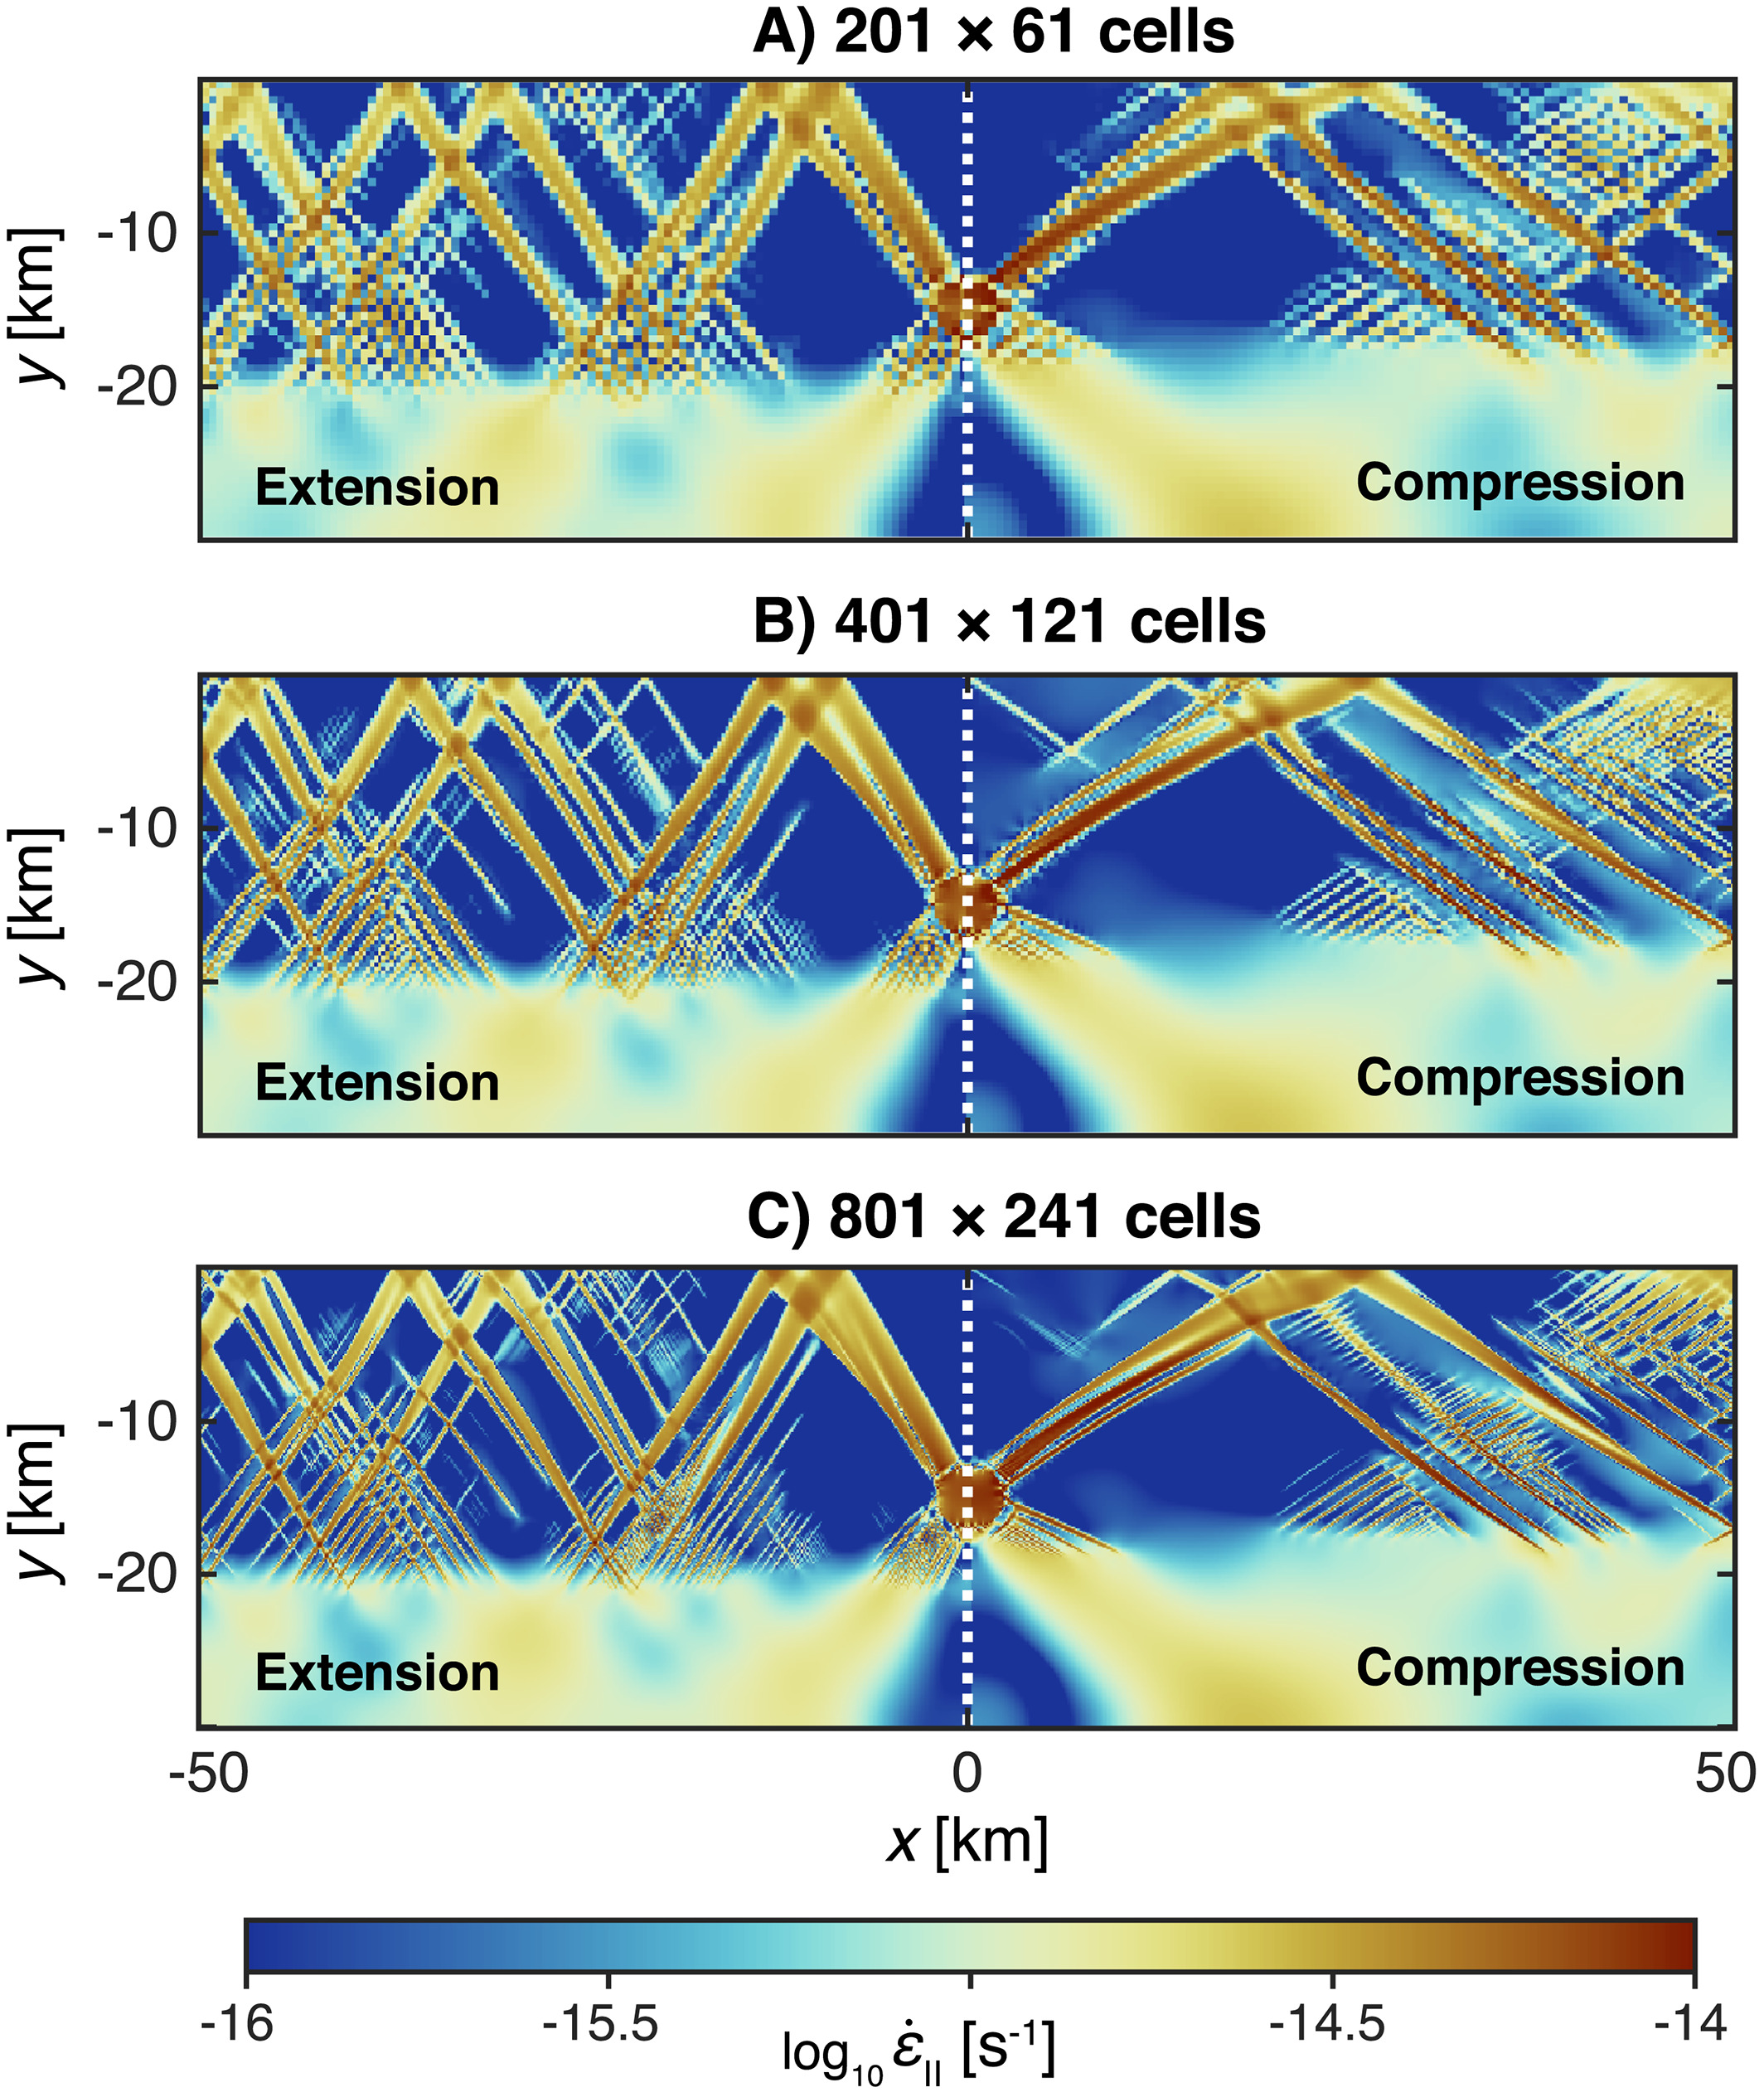
\includegraphics[width=11cm]{python_codes/fieldstone_70/images/fig2}\\
{\captionfont Figure taken from \cite{dudy20}}
\end{center}


\newpage
%......................
\paragraph{Extension}. 

%\begin{center}
%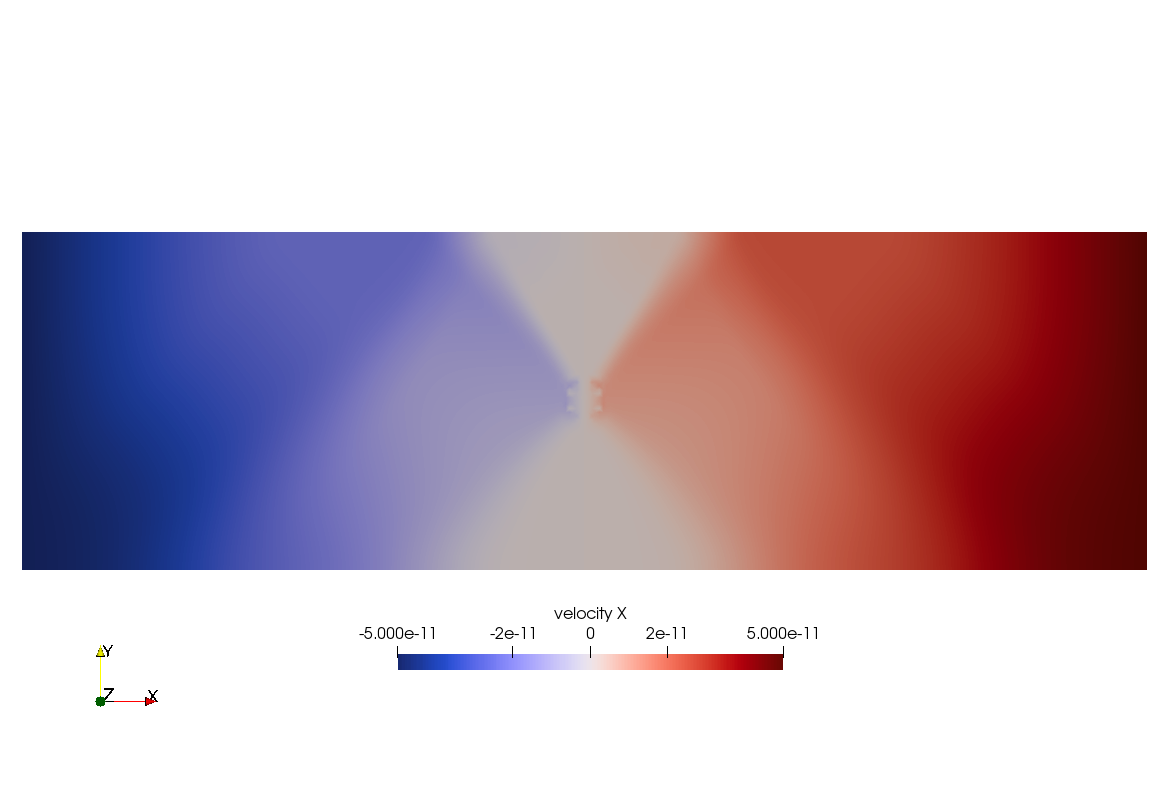
\includegraphics[width=7cm]{python_codes/fieldstone_70/extension/u}
%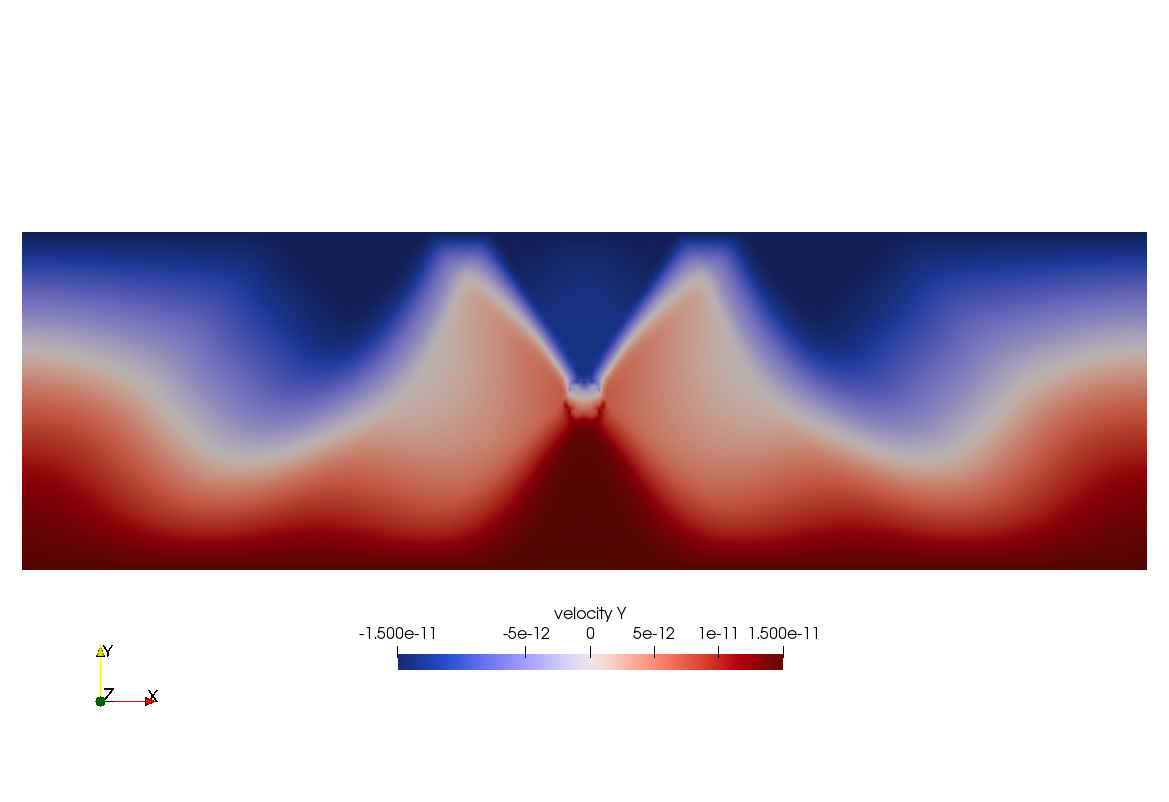
\includegraphics[width=7cm]{python_codes/fieldstone_70/extension/v}\\
%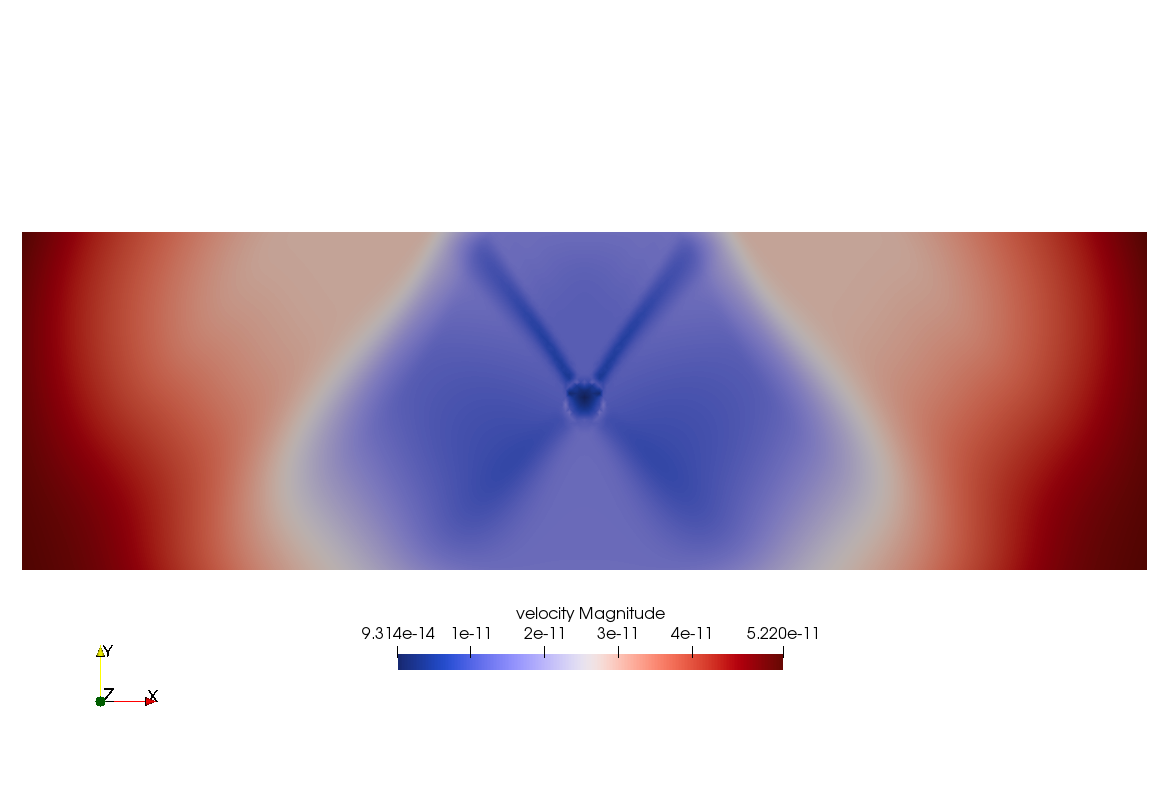
\includegraphics[width=7cm]{python_codes/fieldstone_70/extension/vel}
%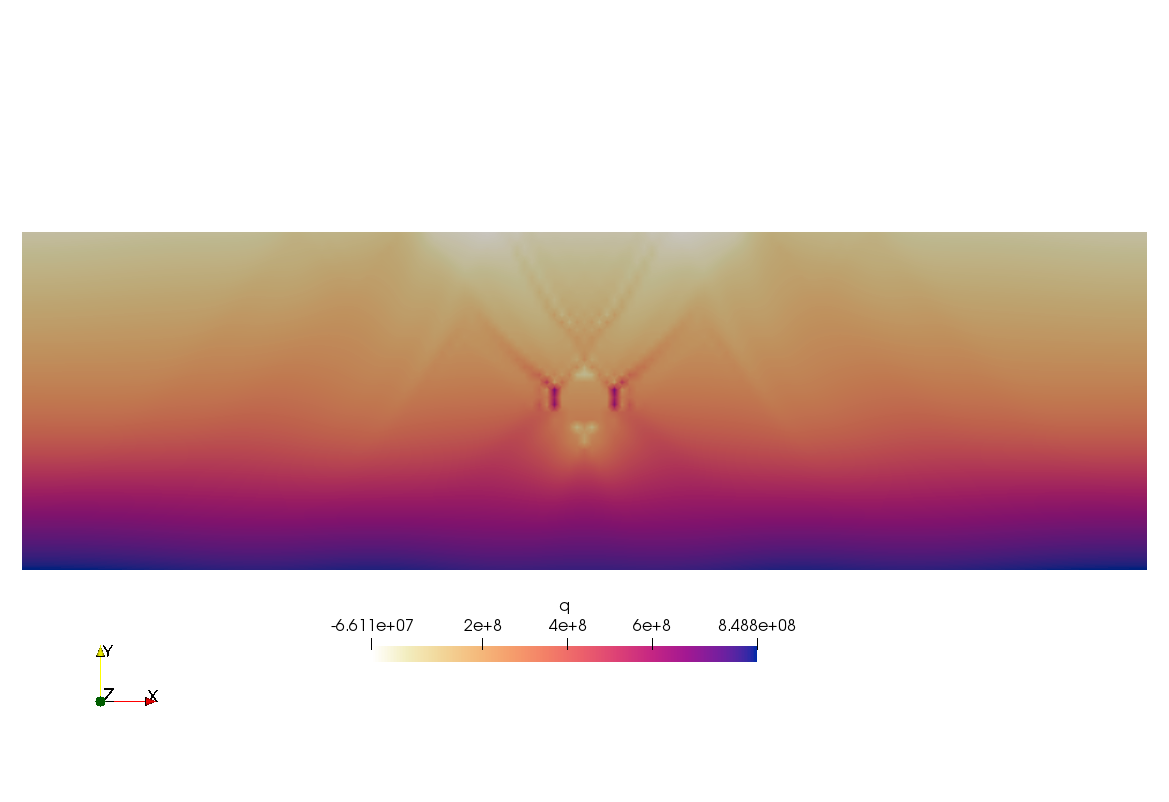
\includegraphics[width=7cm]{python_codes/fieldstone_70/extension/q}\\
%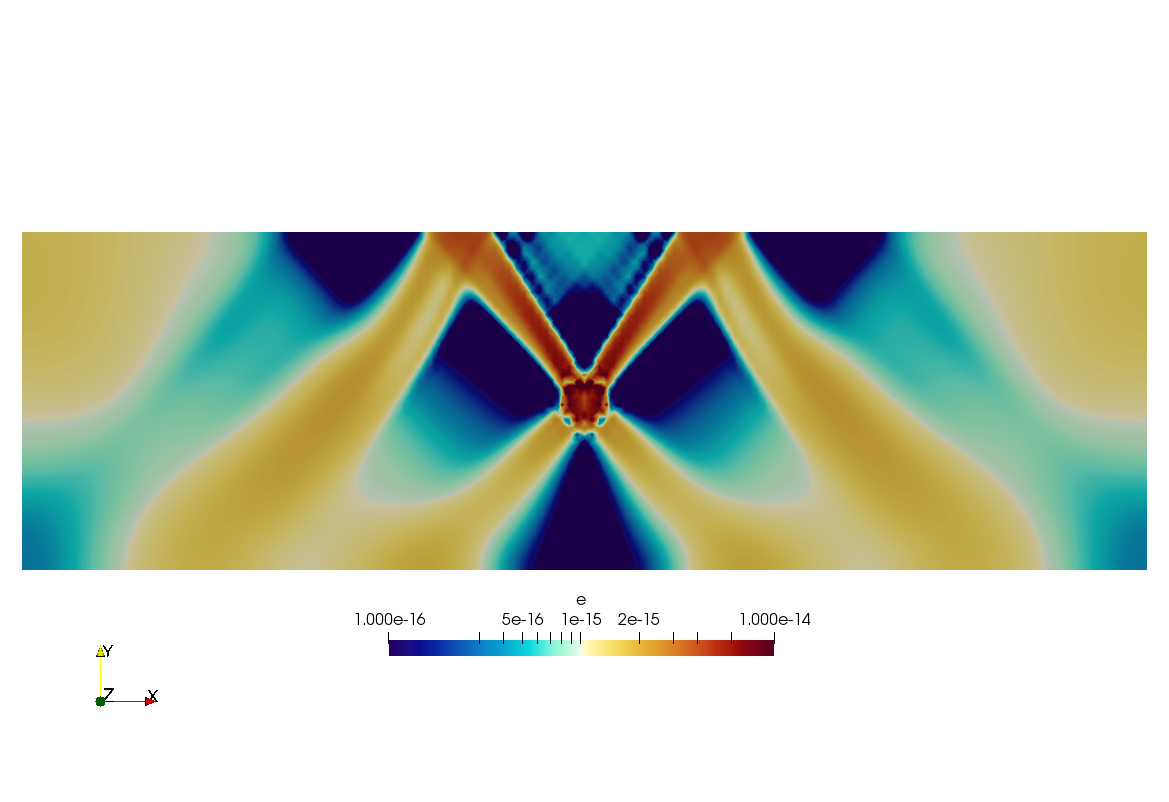
\includegraphics[width=7cm]{python_codes/fieldstone_70/extension/e}
%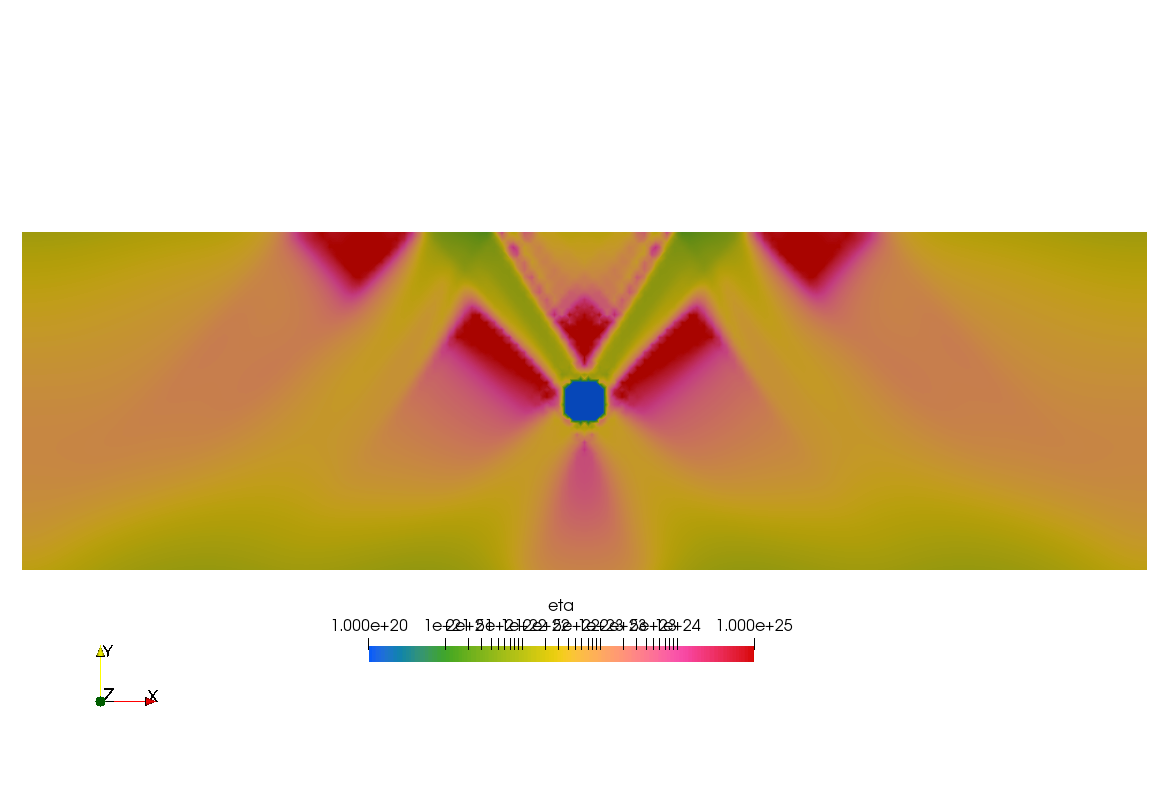
\includegraphics[width=7cm]{python_codes/fieldstone_70/extension/etaeff}\\
%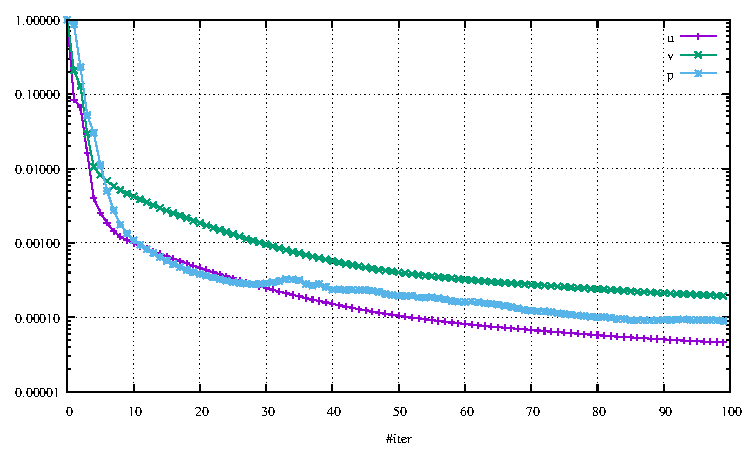
\includegraphics[width=6cm]{python_codes/fieldstone_70/extension/conv.pdf}
%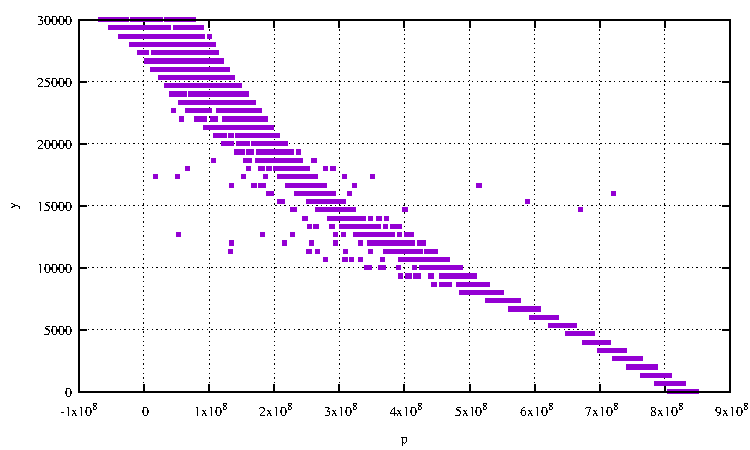
\includegraphics[width=6cm]{python_codes/fieldstone_70/extension/pressure.pdf}\\
%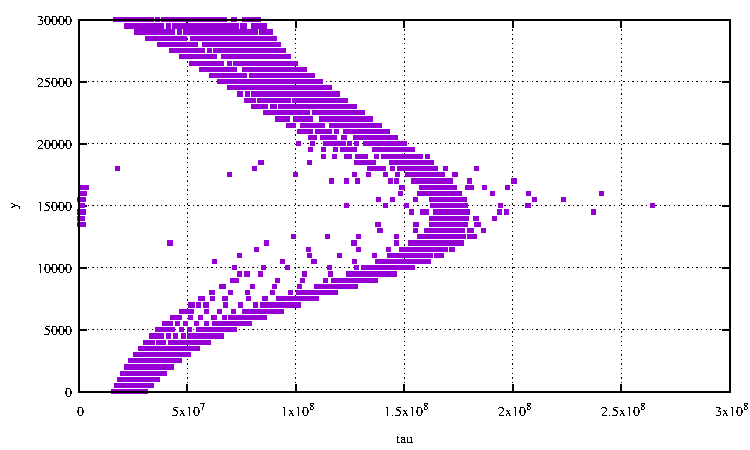
\includegraphics[width=6cm]{python_codes/fieldstone_70/extension/tau.pdf}\\
%extension, resolution 150x45, 100 nl iterations only.
%\end{center}

\newpage
%......................
\paragraph{Compression}. 

%\begin{center}
%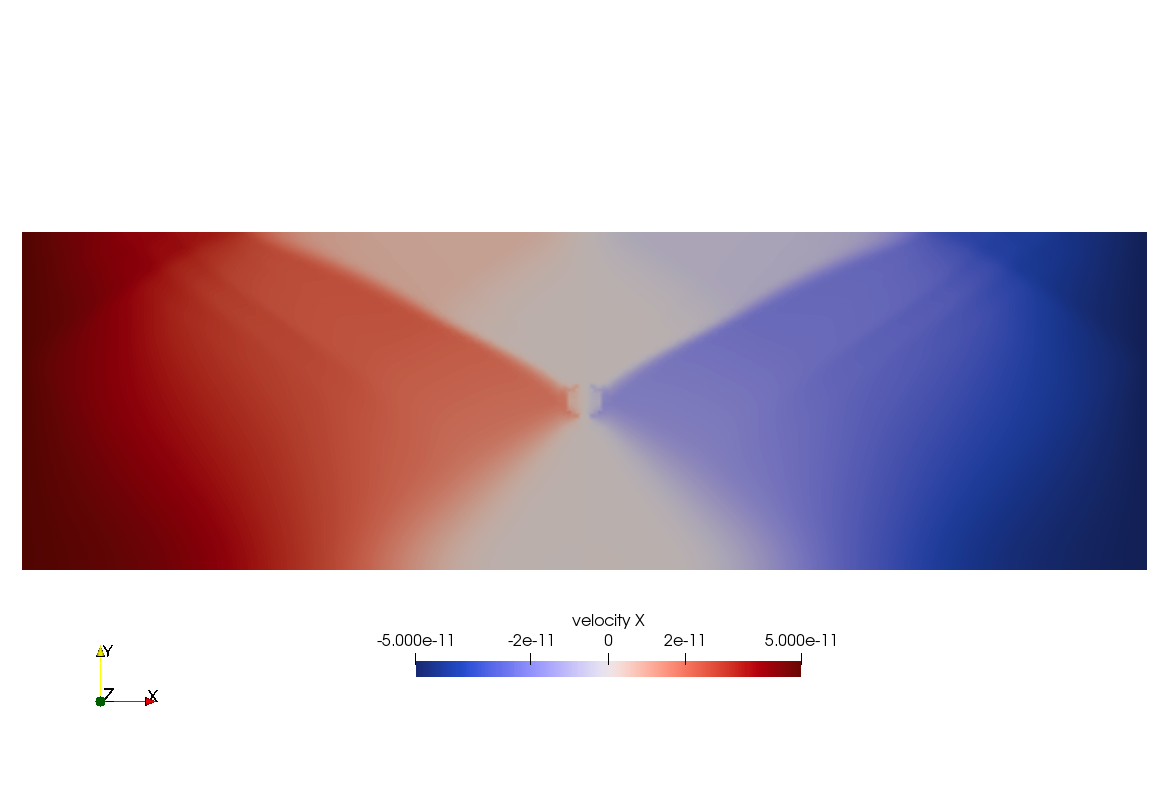
\includegraphics[width=7cm]{python_codes/fieldstone_70/compression/u}
%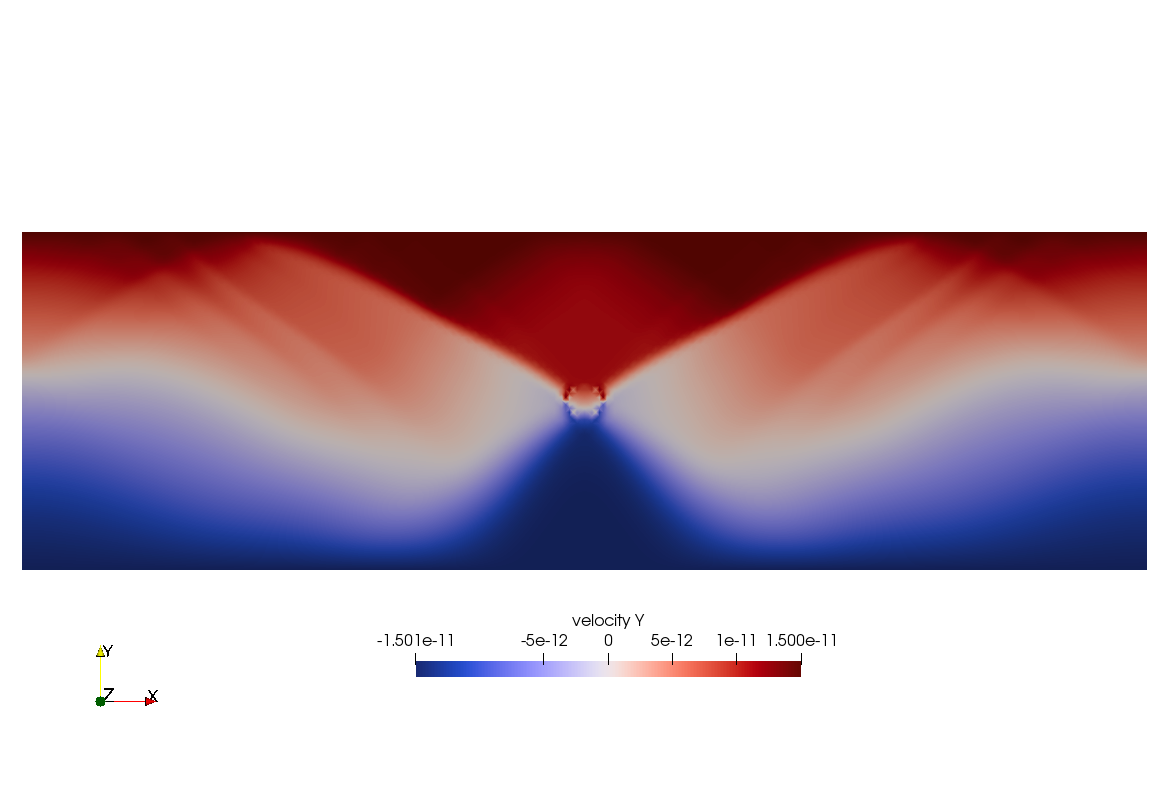
\includegraphics[width=7cm]{python_codes/fieldstone_70/compression/v}\\
%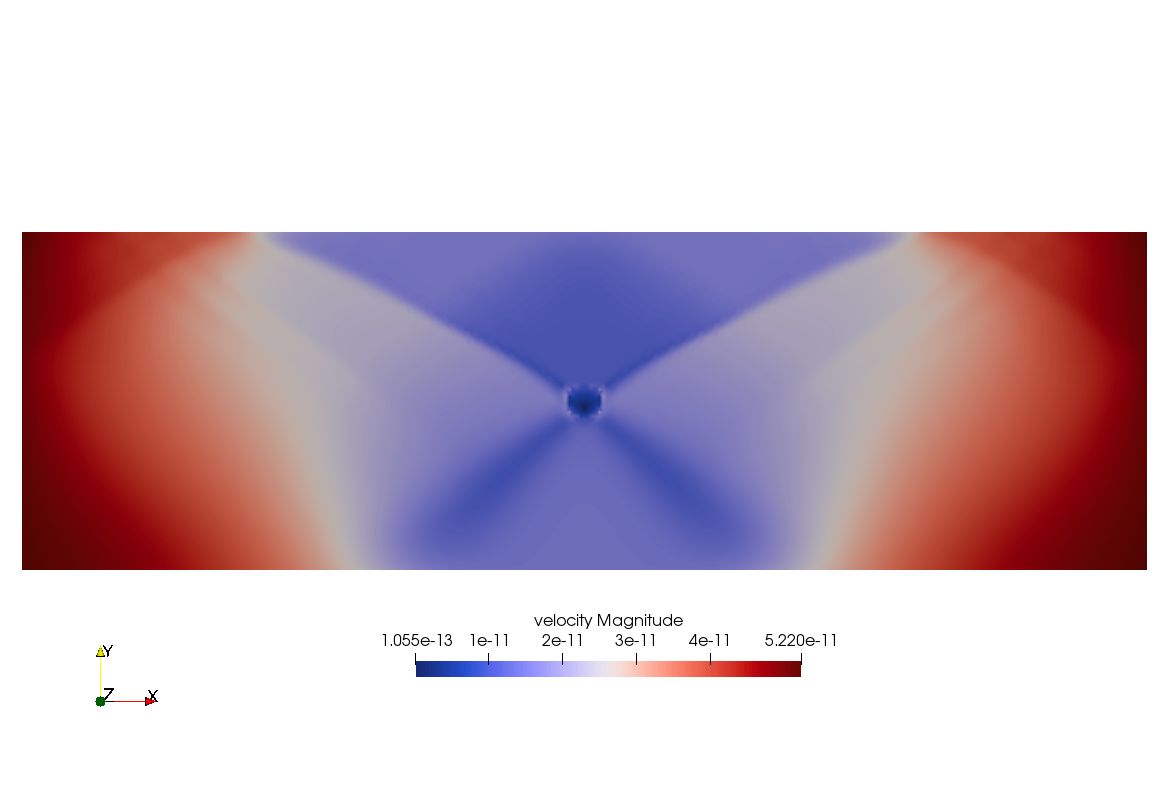
\includegraphics[width=7cm]{python_codes/fieldstone_70/compression/vel}
%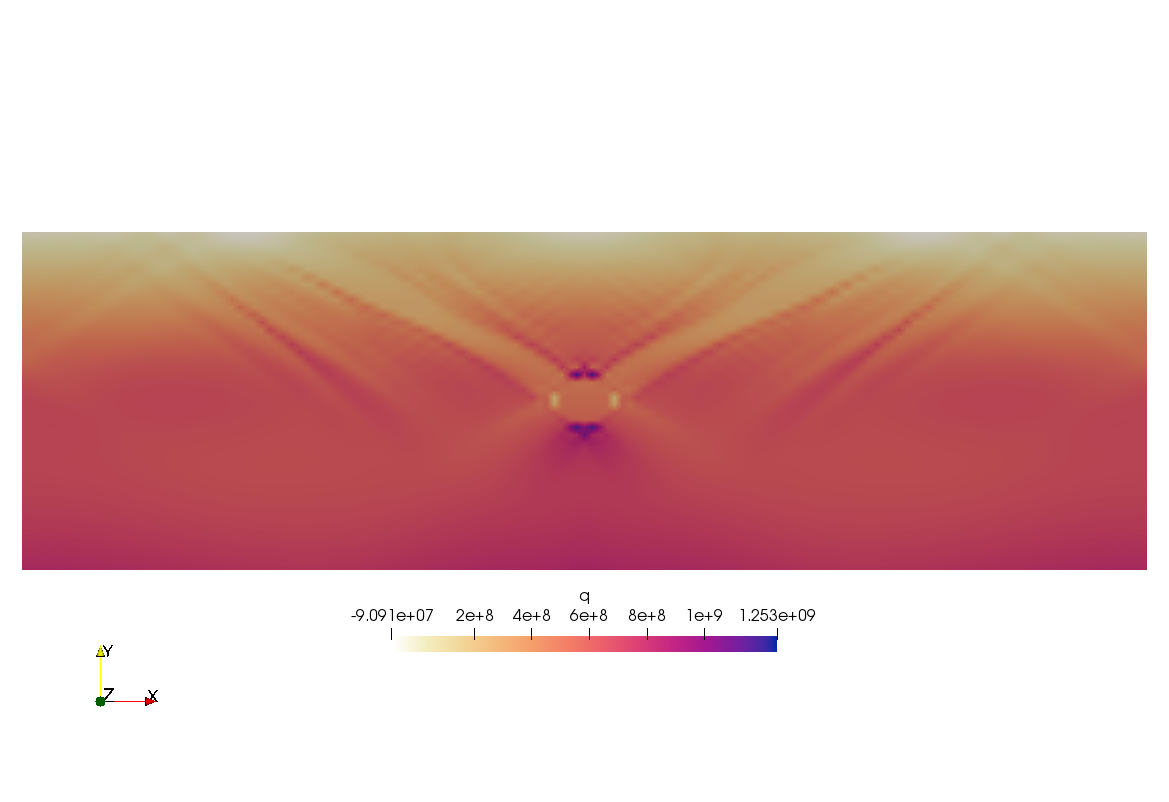
\includegraphics[width=7cm]{python_codes/fieldstone_70/compression/q}\\
%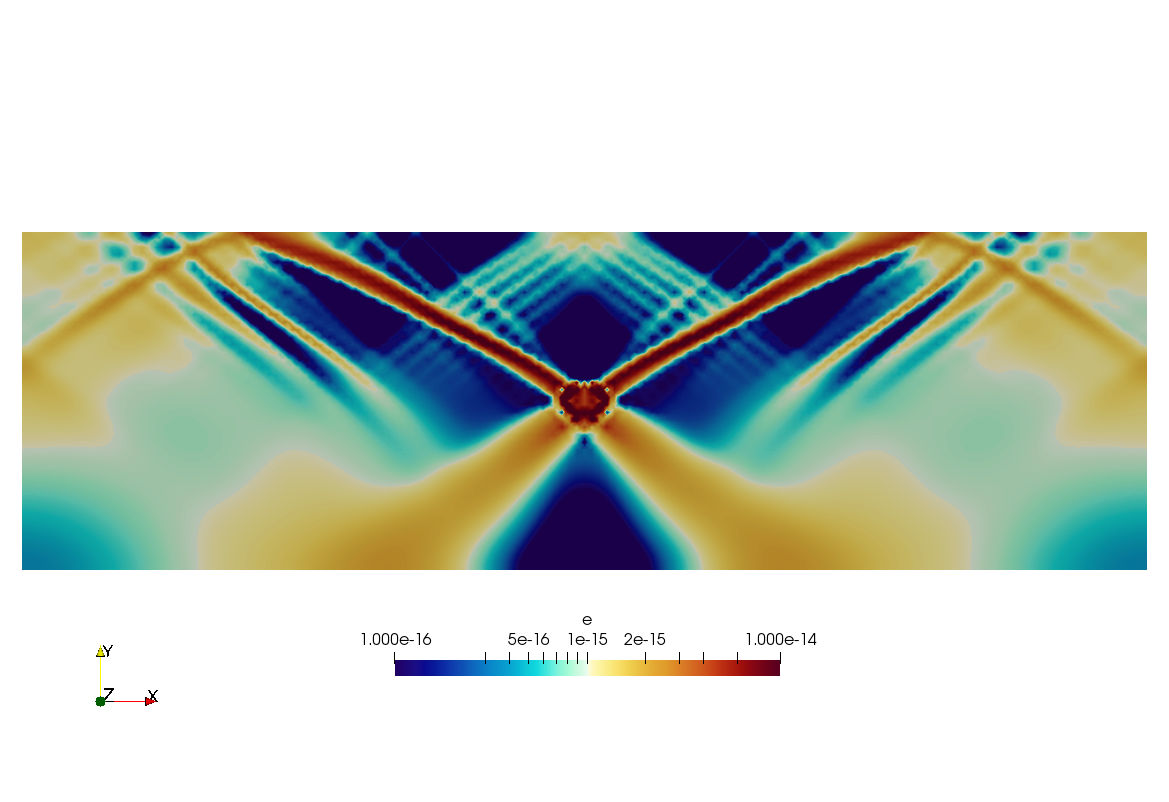
\includegraphics[width=7cm]{python_codes/fieldstone_70/compression/e}
%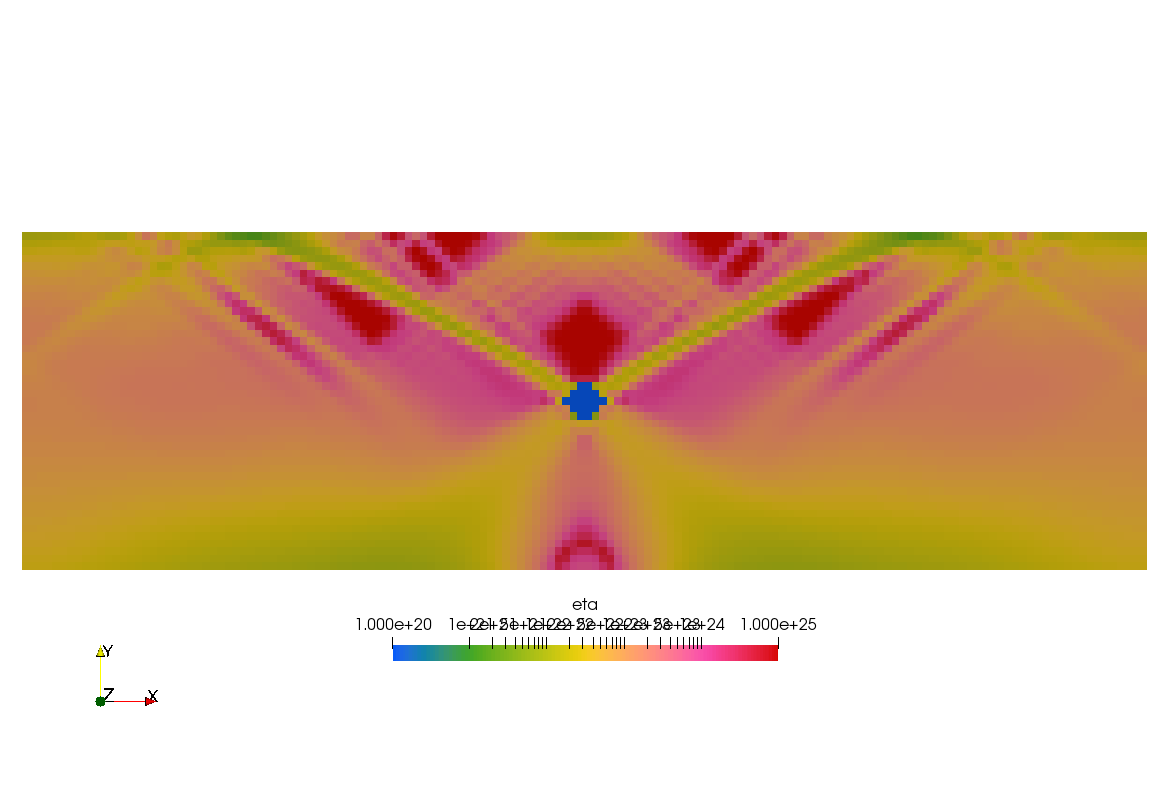
\includegraphics[width=7cm]{python_codes/fieldstone_70/compression/etaeff}\\
%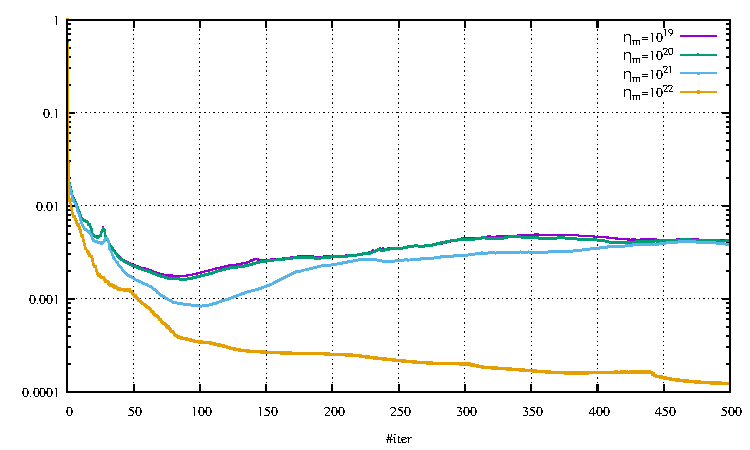
\includegraphics[width=6cm]{python_codes/fieldstone_70/compression/conv.pdf}
%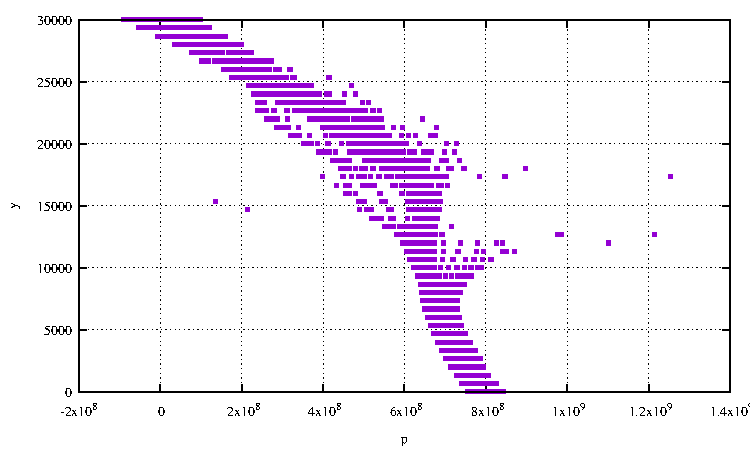
\includegraphics[width=6cm]{python_codes/fieldstone_70/compression/pressure.pdf}\\
%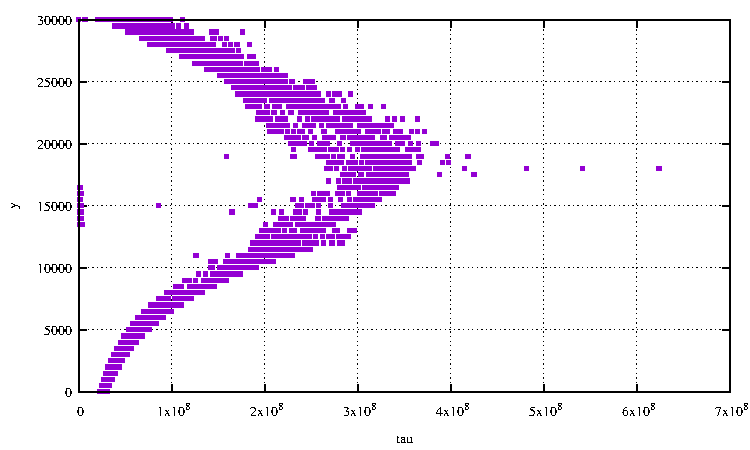
\includegraphics[width=6cm]{python_codes/fieldstone_70/compression/tau.pdf}\\
%extension, resolution 150x45, 100 nl iterations only.
%\end{center}

